%% ======================================================================
%%  IEEE journal paper (IEEEtran, journal mode)
%%
%%  Build:  pdflatex IEEE_paper -> bibtex IEEE_paper -> pdflatex x2
%%  Overleaf: upload this folder (IEEE_paper.tex, references.bib, figures/),
%%            compiler = pdfLaTeX.
%%
%%  Every number in this paper is produced by the scripts in scripts/
%%  (run_inference.py, run_baselines.py, find_duplicates.py,
%%  analyze_leakage.py, make_figures.py) from the trained model
%%  models/taka_authenticator.pth and the public JaalTaka dataset.
%% ======================================================================

\documentclass[journal]{IEEEtran}

\usepackage{cite}
\usepackage{amsmath,amssymb,amsfonts}
\usepackage{graphicx}
\usepackage{booktabs}
\usepackage{adjustbox}
\usepackage{array}
\usepackage{url}
\usepackage{xcolor}
\usepackage[hidelinks,
  pdftitle={Reliable Smartphone-Based Detection of Counterfeit Bangladeshi Banknotes},
  pdfauthor={Debobrato Biswas, Imran Mahmud}]{hyperref}

\graphicspath{{figures/}}
\hyphenation{bank-note bank-notes counter-feit counter-feits Efficient-Net}

\begin{document}

\title{Reliable Smartphone-Based Detection of Counterfeit Bangladeshi Banknotes:
Multi-View Deep Learning with Out-of-Distribution Rejection and a Benchmark Audit}

\author{Debobrato~Biswas and Imran~Mahmud%
\thanks{D. Biswas and I. Mahmud are with the Department of Software Engineering,
Daffodil International University, Dhaka 1207, Bangladesh.}%
\thanks{Corresponding author: Debobrato Biswas (e-mail: biswas2305343003@diu.edu.bd).}}

\markboth{Reliable Smartphone-Based Detection of Counterfeit Bangladeshi Banknotes}%
{Biswas and Mahmud: Reliable Smartphone-Based Detection of Counterfeit Bangladeshi Banknotes}

\maketitle

%% ----------------------------------------------------------------------
\begin{abstract}
\textbf{Background:} Counterfeit high-value banknotes harm retailers and individuals who
cannot afford verification hardware.\\
\textbf{Methods:} We present a smartphone-based authentication system for Bangladeshi
Tk~500 and Tk~1000 notes and evaluate it on JaalTaka, a public benchmark of 1{,}390
notes (802 genuine, 588 seized counterfeits) with six photographs each. The system
fine-tunes EfficientNet-B0, fuses up to six photographs per note, returns a genuine,
uncertain, or counterfeit verdict, rejects unsupported inputs with an embedding-space
test, and explains decisions with Grad-CAM. We audited the benchmark with pixel-level
duplicate matching.\\
\textbf{Results:} On 208 held-out test notes, the system reaches 98.08\% note-level
accuracy (95\% CI 95.16--99.25\%) and an ROC-AUC of 0.994 at 37~ms per photograph on a
CPU. However, the 1{,}390 notes form only 846 distinct photograph sets, 116 test notes
have a copy in training or validation, and 12 duplicate groups carry both labels; all
four test errors fall in these groups. On the 92 test notes without a copy, the system
and two frozen-feature baselines are error-free.\\
\textbf{Conclusion:} The benchmark is saturated under note-level splitting. We release
the duplicate groups and recommend group-aware, counterfeit-family hold-out evaluation.
\end{abstract}

\begin{IEEEkeywords}
Banknote authentication, Bangladeshi Taka, counterfeit detection, data leakage,
EfficientNet, explainable AI, Grad-CAM, out-of-distribution detection, transfer learning.
\end{IEEEkeywords}

\noindent\textbf{Word count:} 2{,}976 words (excluding references); main text: 1{,}932
words; abstract: 186 words.

\section*{Plain Language Summary}
Fake Tk~500 and Tk~1000 notes are hard to spot by eye. We built a tool that checks a
banknote from one to six phone photographs, answers ``genuine'', ``counterfeit'', or
``uncertain'', refuses pictures of other objects, and highlights the parts of the note
behind its answer. It was correct for 98\% of the test notes of a public photo
collection. That collection, however, contains many repeated photographs, some labelled
both genuine and fake, and these explained every mistake. The tool may therefore not
catch new kinds of fakes. We share the repeated photographs and suggest fairer tests.

%% ======================================================================
\section{Introduction}
\label{sec:intro}

\IEEEPARstart{C}{ounterfeit} Tk~500 and Tk~1000 notes undermine trust in cash, the main
means of payment for small retailers in Bangladesh. Banks use ultraviolet, infrared, and
magnetic sorters, but shopkeepers and citizens rely on visual and tactile checks that are
slow and unreliable for untrained users. A smartphone camera, carried by almost
everyone, makes image-based authentication an attractive complement.

The JaalTaka dataset~\cite{piyas2025jaaltaka} enabled such work for Bangladeshi notes by
releasing smartphone photographs of genuine notes and of counterfeits seized by the
Rapid Action Battalion (RAB); its authors reported 97.4--98.9\% accuracy for five
ImageNet CNNs. High benchmark accuracy is necessary but not sufficient for a tool that
people trust with money. It must also (i)~handle unsupported inputs, (ii)~admit
uncertainty, (iii)~explain its decisions, and (iv)~be evaluated in a way that predicts
behaviour on unseen notes. The last point is easy to get wrong: networks exploit
shortcuts~\cite{geirhos2020shortcut}, and duplicates across splits inflate
accuracy~\cite{kapoor2023leakage}. Our contributions are:
\begin{enumerate}
\item an open, CPU-real-time pipeline (Fig.~\ref{fig:pipeline}) combining
EfficientNet-B0~\cite{tan2019efficientnet}, fusion of up to six photographs, a three-way
decision with adjustable strictness, an out-of-distribution (OOD) gate, and
Grad-CAM~\cite{selvaraju2017gradcam};
\item a note-disjoint evaluation with confidence intervals, threshold and OOD analyses,
and frozen-feature baselines; and
\item a duplicate audit showing that label conflicts between copied notes cause every
test error and that the benchmark is saturated, plus an occlusion test revealing signal
outside the note's centre.
\end{enumerate}

\begin{figure*}[!t]
\centering
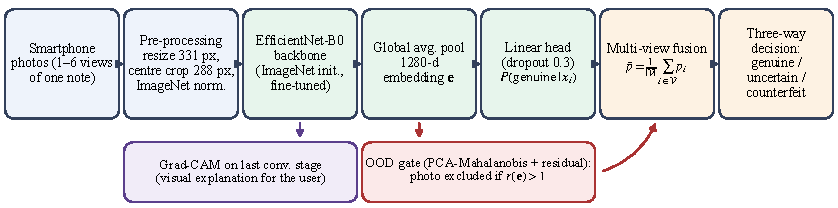
\includegraphics[width=\textwidth]{fig_pipeline}
\caption{Overview of the system. Each photograph is classified by a fine-tuned
EfficientNet-B0; photographs failing the OOD test are excluded, the remaining genuine
probabilities are averaged, and a three-way verdict is returned with Grad-CAM maps.}
\label{fig:pipeline}
\end{figure*}

%% ======================================================================
\section{Related Work}
\label{sec:related}

Early detectors used hand-crafted features: luminance histograms with multiple-kernel
SVMs~\cite{yeh2011}, scanned background printing texture~\cite{berenguel2016}, the
multispectral response of inks~\cite{baek2018}, and individual security features of
Bangladeshi notes~\cite{uddin2016}; a mobile application was also
proposed~\cite{dittimi2018}. These methods depend on controlled imaging and
denomination-specific tuning. Transfer learning from
ImageNet~\cite{deng2009imagenet,yosinski2014transferable} lets CNNs learn from few
images: Pham~\textit{et~al.} detected fake banknotes in smartphone
images~\cite{pham2020,pham2022}, Bangladeshi denominations were recognised with neural
networks and lightweight CNNs~\cite{jahangir2007,linkon2020}, JaalTaka was
benchmarked~\cite{piyas2025jaaltaka} with DenseNet121~\cite{huang2017densenet},
ResNet50~\cite{he2016resnet}, VGG16~\cite{simonyan2015vgg},
MobileNetV2~\cite{sandler2018mobilenetv2}, and InceptionV3~\cite{szegedy2016inception},
and transfer learning was also applied in~\cite{tabassum2025}. None of these studies
evaluates OOD inputs, uncertainty, or duplicates.

Maximum softmax probability is a weak OOD signal~\cite{hendrycks2017baseline};
Mahalanobis distances on network features are stronger~\cite{lee2018mahalanobis}, and
we adapt them to a low-dimensional subspace. Miscalibrated
probabilities~\cite{guo2017calibration} motivate an explicit ``uncertain'' outcome, and
Grad-CAM~\cite{selvaraju2017gradcam} shows the regions supporting a class. Shortcut
learning~\cite{geirhos2020shortcut} and train--test leakage~\cite{kapoor2023leakage}
motivate our audit.

%% ======================================================================
\section{Dataset and Evaluation Protocol}
\label{sec:data}

JaalTaka~\cite{piyas2025jaaltaka,jaaltaka_data} (CC~BY~4.0) contains 1{,}390 notes:
802 genuine (398 Tk~500, 404 Tk~1000) from three national banks and 588 counterfeit
(320 Tk~500, 268 Tk~1000) supplied by RAB. Each note was photographed six times, showing
different segments (Fig.~\ref{fig:samples}), with one of four smartphones (Samsung Galaxy
A50 and M31, Redmi Note~8 and Note~9~Pro), giving 8{,}340 images, which we resized to a
longer side of 1{,}024 pixels. According to the dataset description, 649 original notes
(502 genuine, 147 counterfeit) were expanded to 1{,}390 by augmentation.

\begin{figure*}[!t]
\centering
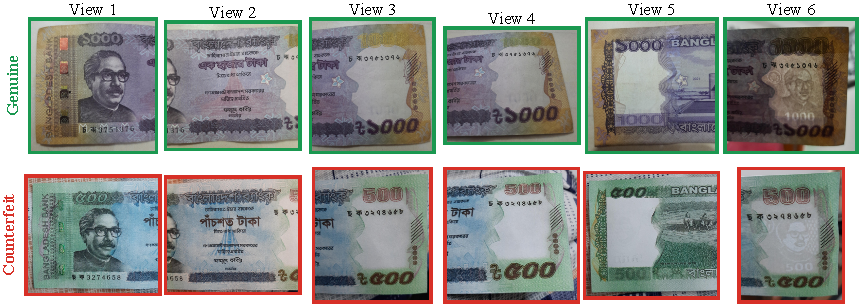
\includegraphics[width=\textwidth]{fig_samples}
\caption{The six photographs of a genuine Tk~1000 note (top) and a counterfeit Tk~500
note (bottom) from the test split; colour, lighting, and background vary with the phone
and session.}
\label{fig:samples}
\end{figure*}

Because the photographs of a note are correlated, we split by note: within each class,
notes were shuffled (seed 42) and assigned 70/15/15\% to training (562 genuine, 412
counterfeit; 5{,}844 photographs), validation, and test (120 genuine, 88 counterfeit;
1{,}248 photographs each). Validation serves model selection and OOD calibration; the test
split is used once. Section~\ref{sec:audit} shows that this note-disjoint split is
\emph{not} sufficient, because distinct notes can share photographs.

%% ======================================================================
\section{Proposed System}
\label{sec:method}

\subsection{Classifier and Training}
\label{sec:training}
EfficientNet-B0~\cite{tan2019efficientnet}, chosen for its accuracy--cost trade-off on
CPUs and initialised with ImageNet weights~\cite{deng2009imagenet}, maps a $288\times288$ input $x$ to a
$1280\times9\times9$ feature map; global average pooling yields the embedding
$\mathbf{e}=f(x)\in\mathbb{R}^{1280}$. The head is dropout ($p=0.3$) and a linear layer:
\begin{equation}
p(x) = \operatorname{softmax}\!\left(\mathbf{W}\mathbf{e}+\mathbf{b}\right)_{\text{genuine}} .
\label{eq:prob}
\end{equation}
The model has 4.01~M parameters. Training uses random resized crops (scale 0.35--1.0,
aspect 0.75--1.33), rotations up to $\pm10^\circ$, colour jitter (brightness and contrast
$\pm0.4$, saturation $\pm0.3$, hue $\pm0.04$), and Gaussian blur ($p=0.2$). At
evaluation, the shorter side is resized to 331 pixels and the central $288\times288$
crop is kept. The stem and first three MBConv stages are frozen with their ImageNet
batch-norm statistics; the rest is fine-tuned with the class-weighted,
label-smoothed~\cite{szegedy2016inception} cross-entropy
\begin{equation}
\mathcal{L} = -\sum_{c\in\{0,1\}} w_c\, q_c \log \hat{y}_c, \quad
q_c = (1-\varepsilon)\,\mathbb{1}[c=y] + \tfrac{\varepsilon}{2},
\label{eq:loss}
\end{equation}
with $\varepsilon=0.05$ and $w_c=N/(2N_c)$. We use AdamW~\cite{loshchilov2019adamw}
(weight decay $10^{-4}$), a one-cycle schedule~\cite{smith2019superconvergence} (peak
$3\times10^{-4}$, 15\% warm-up), batch size 12, and six epochs, keeping the epoch with
the highest validation accuracy plus AUC; accuracy rose from 98.80\% after the first
epoch to 99.04\% (AUC 0.9976) after the sixth, which was selected. Training took
about 55~min on an Intel Core i5-12400 CPU with PyTorch~\cite{paszke2019pytorch}.

\subsection{Multi-View Fusion and Three-Way Decision}
\label{sec:decision}
Let $\mathcal{V}$ be the photographs of a note that pass the OOD gate. The note-level
probability is the mean, a late-fusion form of multi-view pooling~\cite{su2015mvcnn},
\begin{equation}
\bar{p} = \frac{1}{|\mathcal{V}|}\sum_{i\in\mathcal{V}} p(x_i),
\label{eq:fusion}
\end{equation}
and, for a strictness threshold $\tau\in[0.5,1)$ (default 0.7), the verdict is
\begin{equation}
\text{verdict} =
\begin{cases}
\text{not supported} & \text{if } \mathcal{V}=\emptyset,\\
\text{genuine} & \text{if } \bar{p}\ge\tau,\\
\text{counterfeit} & \text{if } \bar{p}<0.5,\\
\text{uncertain} & \text{otherwise.}
\end{cases}
\label{eq:decision}
\end{equation}
Averaging needs no extra training and accepts any number of views. The asymmetry
reflects costs: accepting a counterfeit causes a loss, whereas ``uncertain'' only asks
the user to check the note by hand or add photographs. Users can choose
$\tau\in\{0.6,0.7,0.85\}$ or any other value.

\subsection{Out-of-Distribution Gate}
\label{sec:ood}
Following~\cite{lee2018mahalanobis}, let $\boldsymbol{\mu}$ be the mean training
embedding and $\mathbf{U}_k$ its first $k=64$ principal directions with variances
$\sigma_j^2$. With $\mathbf{z}=\mathbf{U}_k^{\top}(\mathbf{e}-\boldsymbol{\mu})$, we
compute the in-subspace Mahalanobis distance and the out-of-subspace residual
\begin{equation}
m(\mathbf{e}) = \sum_{j=1}^{k}\frac{z_j^2}{\sigma_j^2},\qquad
\rho(\mathbf{e}) = \left\lVert(\mathbf{e}-\boldsymbol{\mu})-\mathbf{U}_k\mathbf{z}\right\rVert_2^2 .
\label{eq:ood}
\end{equation}
Thresholds $\theta_m$ and $\theta_\rho$ are the 99.5th validation percentiles. A
photograph is accepted when
$r(\mathbf{e})=\max\{m/\theta_m,\ \rho/\theta_\rho\}\le1$ and its Laplacian variance (a
texture measure) is at least 30, which rejects blank and blurred images. The residual
catches embeddings that leave the banknote subspace, which the in-subspace distance
alone cannot detect.

\subsection{Explanation and Deployment}
Grad-CAM~\cite{selvaraju2017gradcam} is computed on the last feature map
$A\in\mathbb{R}^{1280\times9\times9}$ for the predicted class $c$:
\begin{equation}
\alpha_k = \frac{1}{81}\sum_{u,v}\frac{\partial y^{c}}{\partial A^{k}_{uv}},\qquad
L^{c} = \operatorname{ReLU}\!\Big(\sum_{k}\alpha_k A^{k}\Big),
\label{eq:gradcam}
\end{equation}
where $y^c$ is the logit of class $c$; the map is normalised, upsampled, and overlaid on
the photograph. The model runs in 37~ms per photograph (median of 30 runs, six CPU threads). The
deployed Flask and Streamlit interfaces also average a full-frame crop; all reported
results use the central crop only.

%% ======================================================================
\section{Experiments and Results}
\label{sec:results}

Genuine is the positive class. We report accuracy with a 95\% Wilson
interval~\cite{wilson1927probable}, the counterfeit detection rate (specificity), the
genuine acceptance rate (recall), and ROC-AUC~\cite{fawcett2006roc}, per photograph
($n=1{,}248$) and per note ($n=208$), at threshold 0.5 unless stated otherwise.

\subsection{Main Results and Baselines}
Per note, the system rejects 86 of 88 counterfeits and accepts 118 of 120 genuine notes
(Table~\ref{tab:main}, Fig.~\ref{fig:confusion}); both ROC curves rise almost vertically
(Fig.~\ref{fig:roc}). The per-note confusion matrix equals the per-photograph matrix
divided by six, and each view position alone reaches 98.08\%: every error comes from all
six photographs of one of four notes.

\begin{table}[!t]
\caption{Test Results of the Proposed System (Threshold 0.5)}
\label{tab:main}
\centering
\footnotesize
\setlength{\tabcolsep}{4pt}
\begin{adjustbox}{max width=\columnwidth}
\begin{tabular}{@{}lcc@{}}
\toprule
Metric & Per photograph & Per note (6 views) \\
\midrule
Samples (genuine / counterf.) & 1{,}248 (720 / 528) & 208 (120 / 88) \\
Accuracy (\%) & 98.08 & 98.08 \\
\quad 95\% Wilson CI (\%) & 97.15--98.70 & 95.16--99.25 \\
Counterfeit detection (\%) & 97.73 & 97.73 (86/88) \\
Genuine acceptance (\%) & 98.33 & 98.33 (118/120) \\
Balanced accuracy (\%) & 98.03 & 98.03 \\
F1, genuine class & 0.983 & 0.983 \\
ROC-AUC & 0.990 & 0.994 \\
\bottomrule
\end{tabular}
\end{adjustbox}
\end{table}

\begin{figure}[!t]
\centering
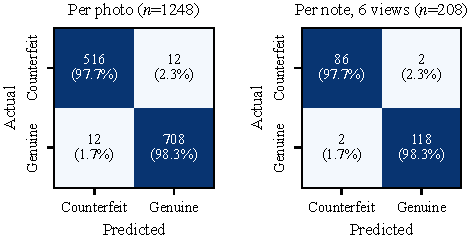
\includegraphics[width=\columnwidth]{fig_confusion}
\caption{Test confusion matrices per photograph (left) and per note (right).}
\label{fig:confusion}
\end{figure}

\begin{figure}[!t]
\centering
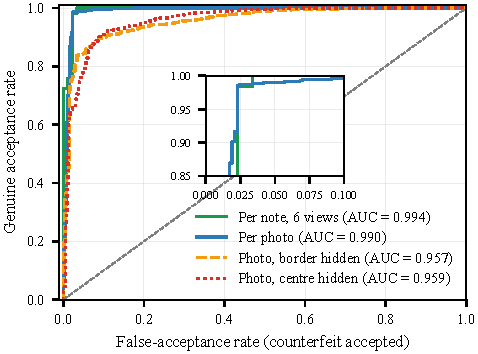
\includegraphics[width=\columnwidth]{fig_roc}
\caption{Test ROC curves for per-note fusion, single photographs, and the occlusion
diagnostics of Section~\ref{sec:shortcut}.}
\label{fig:roc}
\end{figure}

Table~\ref{tab:baselines} compares a cosine 1-nearest-neighbour (1-NN) classifier and a
logistic-regression probe on \emph{frozen} ImageNet EfficientNet-B0 embeddings.
Fine-tuning adds 1.4--1.6 points of per-photograph accuracy, but at note level the probe
matches it and 1-NN errs on only six notes. The JaalTaka authors' results
(97.4--98.9\%~\cite{piyas2025jaaltaka}) used a different split and are not directly
comparable.

\begin{table}[!t]
\caption{Comparison With Frozen-Feature Baselines on the Test Split}
\label{tab:baselines}
\centering
\footnotesize
\setlength{\tabcolsep}{4pt}
\begin{adjustbox}{max width=\columnwidth}
\begin{tabular}{@{}lcccc@{}}
\toprule
& \multicolumn{2}{c}{Per photograph} & \multicolumn{2}{c}{Per note} \\
\cmidrule(lr){2-3}\cmidrule(l){4-5}
Method & Acc.\ (\%) & AUC & Acc.\ (\%) & AUC \\
\midrule
1-NN, frozen ImageNet features & 96.71 & 0.967 & 97.12 & 0.979 \\
Linear probe, frozen features  & 96.47 & 0.981 & 98.08 & 0.983 \\
Fine-tuned EfficientNet-B0 (ours) & \textbf{98.08} & \textbf{0.990} & \textbf{98.08} & \textbf{0.994} \\
\bottomrule
\end{tabular}
\end{adjustbox}
\end{table}

\subsection{Fusion and the Strictness Threshold}
Over all $\binom{6}{k}$ subsets of $k$ views, accuracy stays at 98.08\% while the mean
AUC rises monotonically from 0.9900 ($k=1$) through 0.9912, 0.9917, 0.9925, and 0.9930
to 0.9939 ($k=6$): fusion makes the ranking of notes more reliable. The fused scores are
strongly bimodal (Fig.~\ref{fig:scores}): correctly classified genuine notes have
$\bar{p}>0.86$ and counterfeits $\bar{p}<0.10$, so outcomes are unchanged for
$\tau\le0.85$, and at $\tau=0.90$ one genuine note (0.8\%) becomes ``uncertain''. The two
accepted counterfeits ($\bar{p}\approx0.95$) would need $\tau>0.954$, which would send
most genuine notes to manual inspection.

\begin{figure*}[!t]
\centering
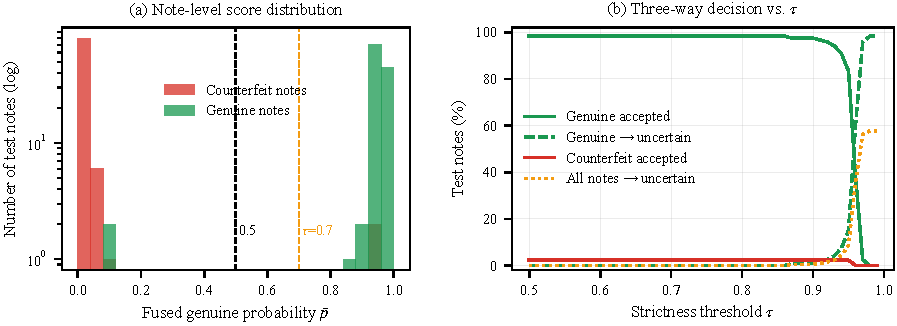
\includegraphics[width=\textwidth]{fig_scores}
\caption{(a) Fused genuine probability $\bar{p}$ of the 208 test notes. (b) Share of
test notes accepted, ``uncertain'', or wrongly accepted versus the threshold $\tau$.}
\label{fig:scores}
\end{figure*}

\subsection{Out-of-Distribution Gate}
The gate rejects 4 of 1{,}248 test photographs (0.32\%) versus 0.72\% on validation, with a
median test ratio of 0.26 (Fig.~\ref{fig:ood}); no test note was ``not supported''. In a
preliminary check, it rejected 100 of 105 photographs of other denominations (Tk~2--200)
and blank, noise, and unrelated images; a systematic OOD benchmark remains future work.

\begin{figure}[!t]
\centering
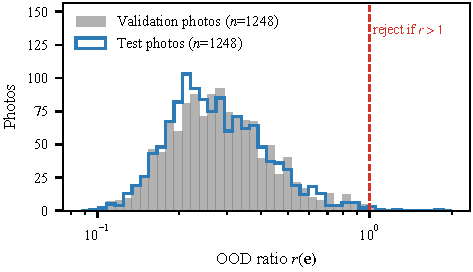
\includegraphics[width=\columnwidth]{fig_ood}
\caption{OOD ratio $r(\mathbf{e})$ of validation and test photographs; the dashed line is
the rejection limit.}
\label{fig:ood}
\end{figure}

\subsection{Visual Explanations}
For correct decisions, Grad-CAM concentrates on the portrait and the denomination and
ornament panels, plus the security band for the counterfeit in Fig.~\ref{fig:gradcam}(b).
The wrongly accepted note in row~(c) looks genuine to the model, as expected because an
identical copy appears in training labelled genuine (Section~\ref{sec:audit}).

\begin{figure*}[!t]
\centering
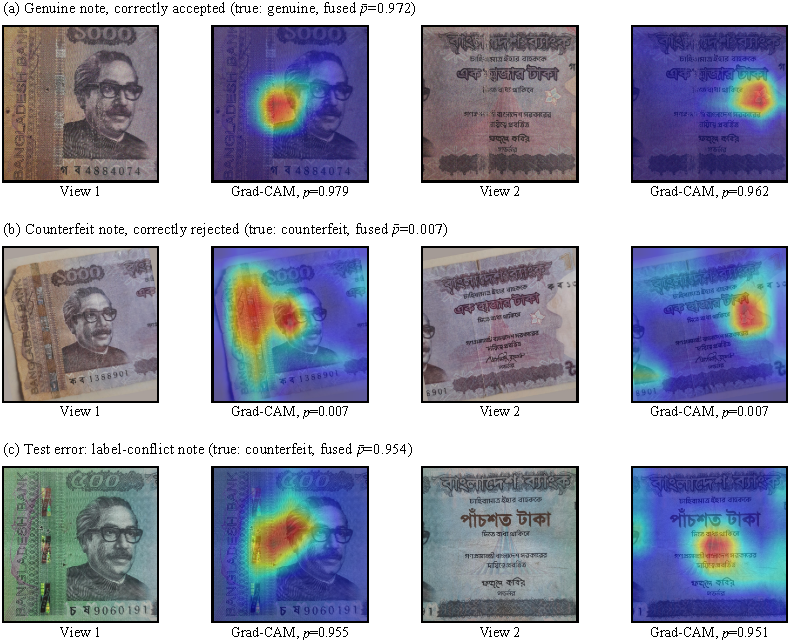
\includegraphics[width=\textwidth]{fig_gradcam}
\caption{Grad-CAM on test notes (views~1 and~2). (a)~Genuine, accepted.
(b)~Counterfeit, rejected. (c)~Counterfeit, wrongly accepted; its photographs occur in
training under the genuine label.}
\label{fig:gradcam}
\end{figure*}

\subsection{Shortcut Diagnostic}
\label{sec:shortcut}
We blacked out either the centre (keeping a 20\% border) or the border of each test input
(Fig.~\ref{fig:shortcut}). Hiding the border gives 88.94\% accuracy (AUC 0.957). Hiding
the centre gives 75.48\%, as most genuine photographs are rejected (acceptance 58.47\%),
yet the AUC remains 0.959 and 98.67\% of counterfeits are recognised. The border, which
holds the note's margins but often also the table or hand beneath it, thus suffices to
rank most photographs.
Because genuine and counterfeit notes came from different sources (banks and RAB),
capture conditions may contribute to decisions~\cite{geirhos2020shortcut}.

\begin{figure*}[!t]
\centering
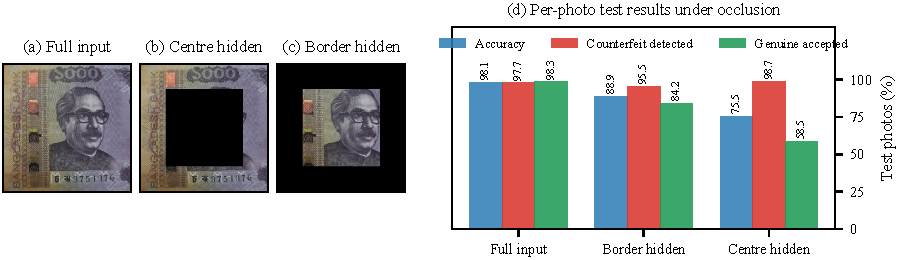
\includegraphics[width=\textwidth]{fig_shortcut}
\caption{Occlusion diagnostic. (a)--(c) Inputs with the centre or the 20\% border
hidden. (d) Per-photograph test results under each condition.}
\label{fig:shortcut}
\end{figure*}

\subsection{Benchmark Audit: Duplicates and Label Conflicts}
\label{sec:audit}
The perfect agreement between a note's photographs, the strong frozen baselines, and
the documented augmentation led us to search for duplicates. For every pair of notes,
we computed the normalised cross-correlation (NCC) of
$48\times48$ grey-scale thumbnails of corresponding views, averaged over the six views
and maximised over flips. The best-match distribution is bimodal
(Fig.~\ref{fig:leakage}(a)): for validation and test notes, no match lies between 0.963
and 0.997. We therefore grouped notes with NCC $>0.98$ (Table~\ref{tab:audit}).

\begin{table}[!t]
\caption{Duplicate Audit of JaalTaka (Pixel NCC $>0.98$ Over Six Views)}
\label{tab:audit}
\centering
\footnotesize
\setlength{\tabcolsep}{4pt}
\begin{adjustbox}{max width=\columnwidth}
\begin{tabular}{@{}lr@{}}
\toprule
Quantity & Value \\
\midrule
Notes / distinct photograph sets (groups) & 1{,}390 / 846 \\
Groups of size 1 / 2 / 3 & 449 / 250 / 147 \\
Notes sharing their photographs with another note & 941 (67.7\%) \\
Groups with only counterfeit / only genuine labels & 289 / 545 \\
Groups containing \emph{both} labels & 12 (31 notes) \\
\midrule
Test notes with a copy in training or validation & 116 of 208 (55.8\%) \\
\quad counterfeit / genuine & 60 of 88 / 56 of 120 \\
Test notes in label-conflict groups & 6 \\
Test errors explained by label conflicts & 4 of 4 \\
\bottomrule
\end{tabular}
\end{adjustbox}
\end{table}

\begin{figure*}[!t]
\centering
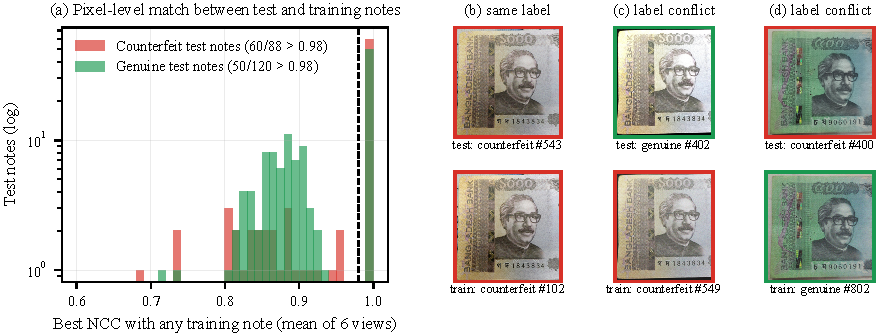
\includegraphics[width=\textwidth]{fig_leakage}
\caption{Duplicate audit. (a) Best NCC match of each test note to any training note;
dashed line: threshold 0.98. (b)--(d) A test note (top) and its matching training note
(bottom); green frame: genuine, red: counterfeit. (b) Augmented copy, same label.
(c), (d) Identical photographs with opposite labels.}
\label{fig:leakage}
\end{figure*}

The augmented copies were thus stored as independent notes, and a note-level split
places copies of 55.8\% of test notes in training or validation. Twelve groups contain
genuine- and counterfeit-labelled copies of the \emph{same} photographs (e.g., genuine
notes 400--406 duplicate counterfeit notes 106--112 and 547--553, and counterfeit notes
400 and 403--406 duplicate genuine notes 802 and 1--4), so at least one label
per group is wrong; genuine-labelled notes 402 and 403 carry serial number 1843834,
which also appears on counterfeit-labelled notes. \emph{All four} test errors are notes
from these groups, each predicted with the label of its training copy. On the 92
\emph{clean} test notes, whose group has no member in training or validation, and on the
202 notes outside label-conflict groups, all three methods are error-free
(Table~\ref{tab:clean}). The 98.08\% accuracy is thus limited by label noise, not by the
model, and the task is saturated even for 1-NN on generic features.

\begin{table}[!t]
\caption{Note-Level Accuracy (\%) on Audited Test Subsets}
\label{tab:clean}
\centering
\footnotesize
\setlength{\tabcolsep}{4pt}
\begin{adjustbox}{max width=\columnwidth}
\begin{tabular}{@{}lccc@{}}
\toprule
Test subset & All & Without label & Clean \\
& & conflicts & (no copy) \\
\midrule
Notes (genuine / counterf.) & 208 (120/88) & 202 (117/85) & 92 (64/28) \\
\midrule
1-NN, frozen features & 97.12 & 100.0 & 100.0 \\
Linear probe, frozen & 98.08 & 100.0 & 100.0 \\
Ours (fine-tuned) & 98.08 & 100.0 & 100.0 \\
\quad 95\% Wilson CI & 95.16--99.25 & 98.13--100 & 95.99--100 \\
\bottomrule
\end{tabular}
\end{adjustbox}
\end{table}

%% ======================================================================
\section{Discussion}
\label{sec:discussion}

Within JaalTaka, the system is error-free once label conflicts are removed (lower 95\%
bound 96.0\% on the 92 clean notes), its errors are fully explained, and it runs in real
time on a CPU. This does not show that it will detect \emph{new} counterfeits: the 588
counterfeits collapse into 289 photograph sets, those we inspected share a few serial
numbers, and they were collected separately from the genuine notes. A model, even 1-NN,
can therefore succeed by recognising known batches or capture sessions, as the occlusion
test suggests. The saturated benchmark also cannot rank methods, since differences
between published CNNs are smaller than its label noise.

We recommend (i)~removing or relabelling the 12 conflict groups; (ii)~splitting by
duplicate group, for which we release our list; (iii)~holding out counterfeit families
(e.g., by serial number or seizure batch) and capture devices, to measure generalisation
to unseen forgeries and phones; and (iv)~reporting confidence intervals and
frozen-feature baselines, which immediately reveal saturation.

\textit{Limitations:} The system covers only Tk~500 and Tk~1000. Visible-light
photographs cannot capture ultraviolet, magnetic, or tactile features, so the output is
decision support and suspicious notes should be confirmed at a bank. Scans and distant
photographs are mostly rejected, the OOD evaluation is preliminary, and probabilities
are not calibrated on independent data~\cite{guo2017calibration}. Retraining on a
group-aware split with a counterfeit-family hold-out is the most important next step.

%% ======================================================================
\section{Conclusion}
\label{sec:conclusion}

Our smartphone system combines multi-view fusion, a three-way decision, an OOD gate, and
Grad-CAM, runs in real time on a CPU, and reaches 98.08\% note-level accuracy (AUC 0.994)
on JaalTaka. The audit shows that label conflicts among duplicated notes explain every
error and that on duplicate-free notes even simple baselines are error-free. Progress now
depends on evaluation data that separates counterfeit families, sessions, and devices.

%% ======================================================================
\section*{Acknowledgment}
The authors thank the Department of Software Engineering, Daffodil International
University, for its support and the JaalTaka creators for releasing their data.

\section*{Funding}
This research received no external funding.

\section*{Author Contributions}
D.~Biswas: conceptualisation, software, experiments, analysis, and original draft.
I.~Mahmud: supervision, methodology review, and manuscript editing.

\section*{Conflict of Interest}
The authors declare no conflict of interest.

\section*{Ethics Statement}
This study involved no human participants, personal data, or animals; it used only
banknote photographs from a public CC~BY~4.0 dataset~\cite{jaaltaka_data}. Ethics
approval and informed consent were therefore not required.

\section*{Generative AI Disclosure}
%% TODO (authors): adapt this statement to the journal's policy and to how AI tools
%% were actually used.
The authors used an AI assistant to help write analysis scripts and edit the text, and
checked all code, results, and references.

\section*{Data Availability}
JaalTaka is available from Mendeley Data~\cite{jaaltaka_data}. The model, code, and
duplicate-group list are available from the corresponding author and will be released
publicly upon publication.

%% ----------------------------------------------------------------------
\bibliographystyle{IEEEtran}
\bibliography{references}

%% ----------------------------------------------------------------------
%% Biographies. TODO (authors): complete them, or delete this block if the
%% journal does not ask for biographies. To add a photo, use
%% \begin{IEEEbiography}[{\includegraphics[width=1in,height=1.25in,clip,keepaspectratio]{photo.jpg}}]{Name}
\begin{IEEEbiographynophoto}{Debobrato Biswas}
is with the Department of Software Engineering, Daffodil International University,
Dhaka, Bangladesh. % TODO: degrees, research interests, IEEE membership.
\end{IEEEbiographynophoto}

\begin{IEEEbiographynophoto}{Imran Mahmud}
is with the Department of Software Engineering, Daffodil International University,
Dhaka, Bangladesh. % TODO: degrees, positions, research interests.
\end{IEEEbiographynophoto}

\end{document}
